\documentclass[]{article}
\usepackage{fancyhdr}
\usepackage{graphicx}
\graphicspath{{./latex_imgs/}}


%opening
\title{APCS project, A.Y. 2019-2020\\Project proposal \#50:"Development of an interactive 2D application with  OpenFrameworks"}
\author{Antonio Pipita}

\begin{document}

\maketitle
\newpage
\tableofcontents
\newpage
\section{Introduction}
This project consists in developing an application that enables the user to interact with a 2D environment via video feed.\\
In particular, the user will control via hand motion a component of a simple game: the goal of the player is to destroy a brick wall by making a ball bounce into it, while avoiding to make the ball fall off the screen. In order to do so, the player will move a bar at the bottom of the playfield via motion control.\\
The video feed will be captured via a Microsoft Kinect, mod. 1414\\
\section{Application architectural overview}
This section introduces the application outlining its structure and the information flow.
\subsection{Design pattern}
\begin{figure}[h!]
    \centering
    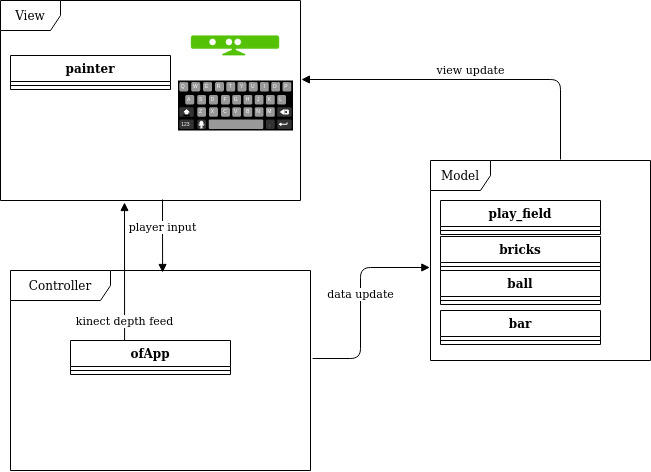
\includegraphics[width=\textwidth]{MVC_mod.jpg}
    \caption{a nice plot}
    \label{fig:MVC}
\end{figure}

\newpage
This application has been designed following the Model-Controller-View pattern:
\begin{itemize}
	\item [Model]: contains the application data and manages its update. In this application it comprehends the classes play\_field, ball, bar and brick.\\
				It manages the movement of the ball on the playfield, its interactions with the bricks, the bar and the playfield edges. It also recives the updates on the bar position and angle, if the required action is possible. 
	\item [Controller]: manages the flow of information from the view to the controller. In this application it comprehends the class ofApp, which grabs input from the kinect device, re-elaborates it and pushes it to the model.
	\item [View]: manages the interaction with the user. In this application it comprehends the painter class, which represents on the device screen the status of the model, partially the ofApp class, since it directly draws the kinect's depth view on the screen, and the hardwar used by the user for the inputs, which comprises the kinect itself and the keyboard. 
\end{itemize}
The splitting of the view between the painter class and the ofApp class was done in order to keep the kinect interaction just in the ofApp class, thus keeping the code a bit more tidy.
\subsection{Development approach}
A bottom-up approach has been chosen for the devvelopment, united with the divide et impera paradigm
\subsection{Testing}
Testing has been performed using VSCode and intellisense debugging, focusing on limit cases 
\subsection{Development environment}
The project has been developed in an Ubuntu environment (Bionic Beaver), using VScode with C/C++ extensions and Intellisense to write, debug and test the code. 
\subsection{Information flow}
The information that the user want to transmit enters the application via the view (kinect and keyboard), is then interpretedd and restructured by the controller and passed to the model. The model applies the requiredd changes to the data, updates itself following the rules of ball movement and then send the new infto the view again, which will print on the screen the current state of the game and give the user new information.\\
\subsection{Phases}
The application works in three different phases:
\begin{itemize}
	\item [Setup phase] this is the phase in which the application starts. During this phase the user can regulate the kinect angle and move on to the game phase.
	\item  [Game phase] in this phase the user plays the actual game. The phase ends when the player finishes all of its lives or destroys all the bricks. Once this phase ends the application moves on to the endgame phase.
	\item [Endgame phase] in this phase the user can either exit the application or play again, thus returning to the setup phase. 
\end{itemize}
\subsection{Acronyms and conventions}
\begin{itemize}
	\item [OF] openframeworks
	\item [playfield] while referring to the class ofApp is used to address the omonimous field of the class; outsidde of the class scope however it is used to refer to all the data relative to the state of the model.
\end{itemize}
\newpage
\section{Classes overview}
This section contains the class diagram and a description of the attributes and methods of each class
\begin{figure}[h!]
    \centering
    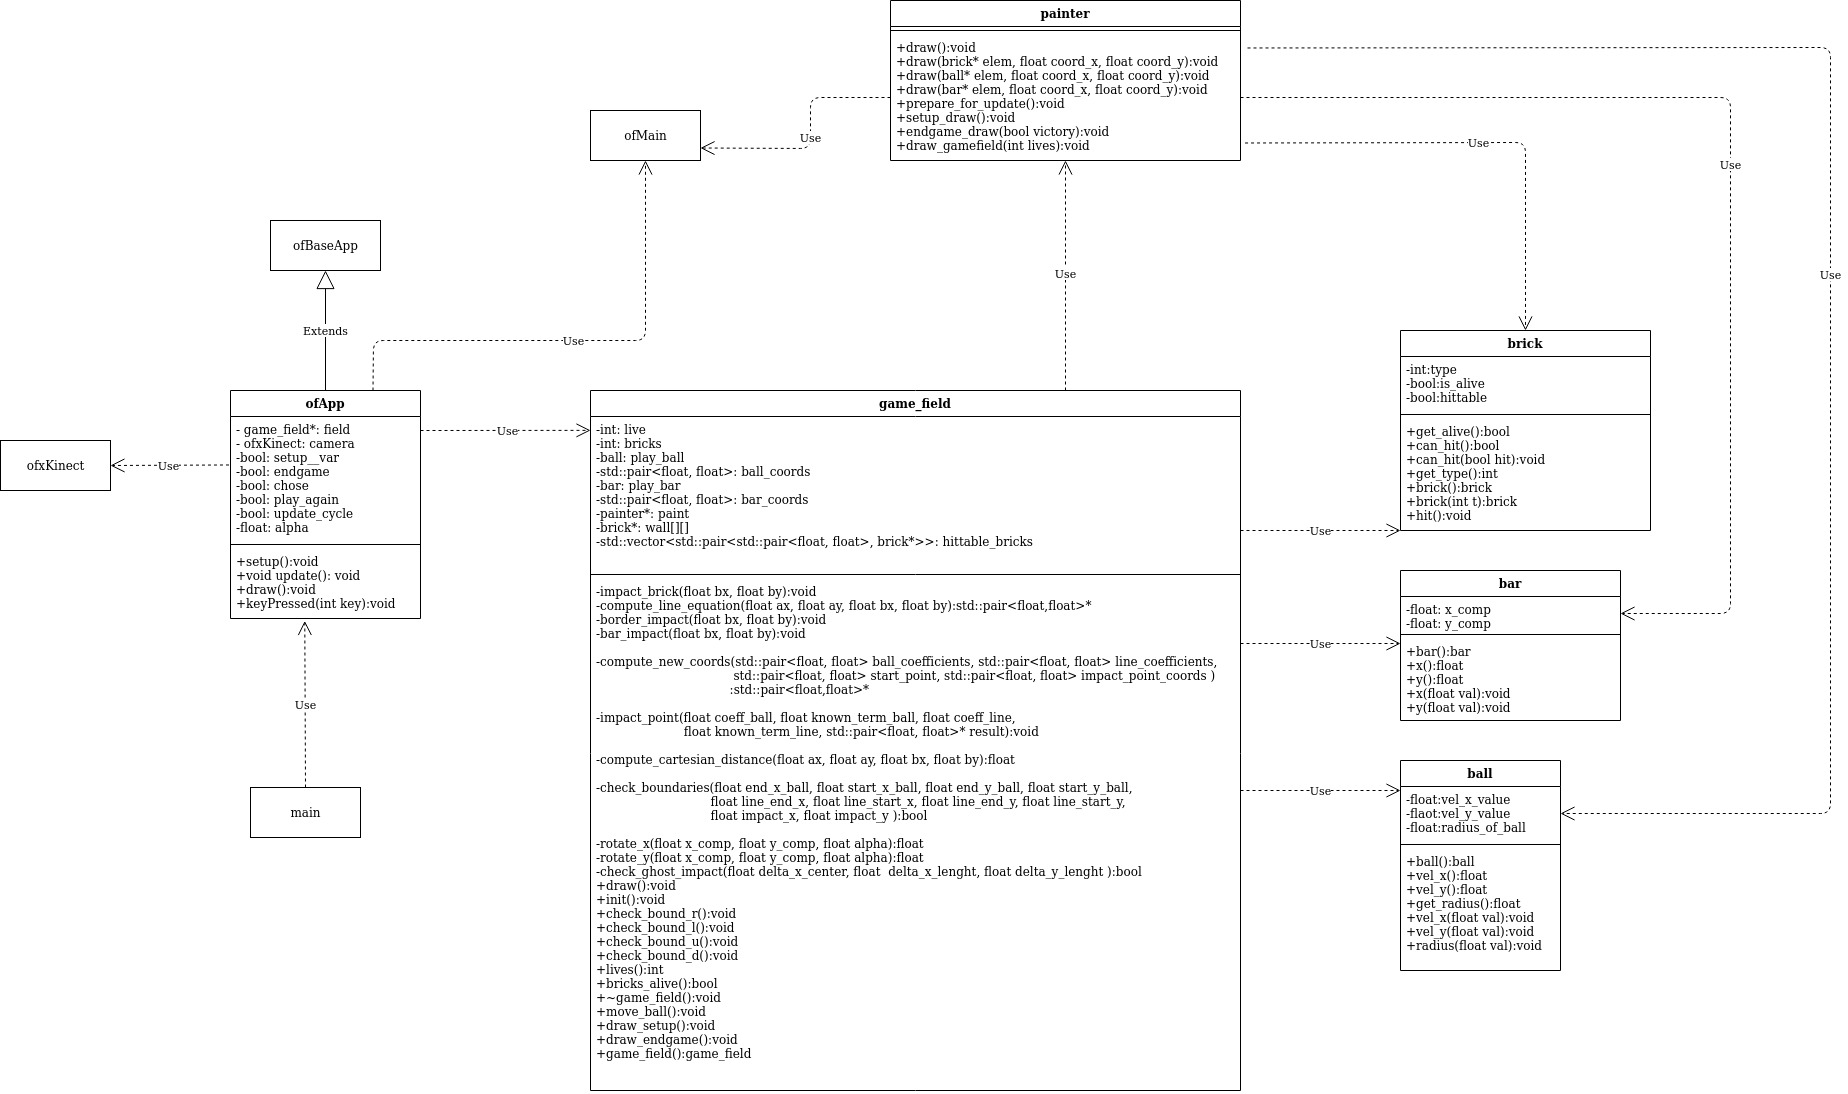
\includegraphics[angle=90, scale=0.25]{calss_diagram_mod.jpg}
    \caption{The class diagram of the application}
    \label{fig:Class diagram}
\end{figure}

\subsection{ofApp}
The ofApp class acts as controller, extends ofBaseApp and is the class upon which the framework provided by OF acts, thus controlling the applicaiton execution.
\begin{figure}[h!]
    \centering
    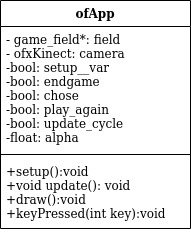
\includegraphics[scale=0.5]{ofApp.jpg}
    \caption{The ofApp class}
    \label{fig:ofApp class diagram }
\end{figure}
\subsubsection{Attributes}
All of the following attributes are private
	\begin{itemize}
		\item game\_field* playfield\\Pointer to the game\_field instance that is currently active, enables the interaction between controller and model.
		\item ofxKinect camera\\The instance of ofxKinect we refer to in order to grab the Kinect feed.
		\item bool setup\_\_var\\Boolean variable used to represent wether the application is in the setup state.
		\item bool endgame\\Boolean variable used to represent wether the application is in the endgame state.
		\item bool chose\\Boolean variable used to represent wether the player has chosen to play again or hasn't taken that decision yet.  
		\item bool play\_again\\Boolean variable used to represent the preference of the player regarding playing again or exiting the application.
		\item bool update\_cycle\\Switch used to choose wether to update the bar state or the ball state.
		\item float alpha\\Kinect angle.
	\end{itemize}
\subsubsection{Methods}
All of the following methods are public
	\begin{itemize}
		\item setup():void \\ Prepares the application for the execution, initializing the playfield, applying settings for the view and establishing a connection with the Kinect.
		\item update():void \\ Main cycle of the application, its behaviour changes according to the game state:
			\begin{itemize}
				\item Setup phase: waits for player input to start the game.
				\item Game phase: asks the model to update the bar state according to the player's input and to update the playfield state according to the rules of the playfield.
				\item Endgame phase: waits to the player's deccision to either exit the game or to play another round; then enforces that decision.
			 \end{itemize}
		\item draw():void \\ Method used to update the graphic representation of the game state, mostly by communicating to the model that it's time to do so. Its behaviour changes according to the game state:
			 \begin{itemize}
				 \item Setup phase: tells the model to print the setup information and provides the Kinect's depth view feed.
				 \item Game phase: tells the model to update the visual representation of thee playfield state.
				 \item Endgame phase: tells the model to print the endgame information.
			 \end{itemize}
		\item keyPressed(int key):void \\ Manages the player's input via keyboard, changes its behaviuor according to the game phase
			 \begin{itemize}
				\item Up key: in the setup phase is used to increment the Kinect's angle, in the endgame phase to choose to play again.
				\item Down key: in the setup phase is used to decrement the Kinect's angle, in the endgame phase to exit the application.
				\item Right key: used only in the setup phase to start playing. 
			 \end{itemize}
	\end{itemize}
\newpage
\subsection{Painter}
\begin{figure}[h!]
    \centering
    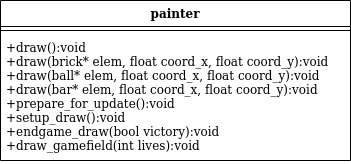
\includegraphics[scale=0.5]{painter.jpg}
    \caption{The painter class}
    \label{fig:painter class diagram }
\end{figure}
This class is used to print to the screen the playfield state representation and the information the user needs. It's composed by public methods:
\begin{itemize}
		\item draw():void \\ General draw method.
		\item draw(brick* elem, float coord\_x, float coord\_y):void\\ Draws a brick.
		\item draw(ball* elem, float coord\_x, float coord\_y):void\\ Draws the ball.
		\item draw(bar* elem, float coord\_x, float coord\_y):void\\ Draws the bar.
		\item prepare\_for\_update():void\\ Clears the screen.
		\item setup\_draw():void\\Draws the setup information.
		\item endgame\_draw(bool victory)\\Draws the endgame information.
		\item draw\_gamefield(int lives):void\\Draws the gamefield boundaries, the number of lives and other information.
	\end{itemize}
It is worth noting that, while this class does not have any attribute, it presents hoever some global variables (situated in the .cpp file) used for the visual representation coordinates computation.
\newpage
\subsection{Brick}
\begin{figure}[h!]
    \centering
    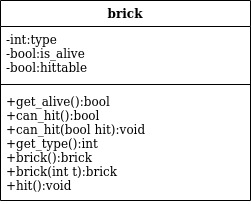
\includegraphics[scale=0.5]{brick.jpg}
    \caption{The brick class}
    \label{fig:brick class diagram }
\end{figure}
This class represents the bricks
\subsubsection{Attributes}
All of the class attributes are private
\begin{itemize}
	\item int:type\\Represents the remaining hitpoints of the brick.
	\item bool:is\_alive\\Represents wether the brick has any hitpoints left.
	\item bool:hittable\\Represents wether the brick is currently reachable by the ball. 
\end{itemize}
\subsubsection{Methods}
All of the class methods are public
\begin{itemize}
	\item get\_alive():bool\\ is\_alive getter.
	\item can\_hit():bool\\hittable getter.
	\item get\_type():int\\ type getter.
	\item can\_hit(bool hit):void\\hittable setter.
	\item hit():void\\ Method called when the brick gets hit.
	\item brick():brick\\Default constructor.
	\item brick(int t):brick\\Constructor that sets the type to t.
\end{itemize}
\subsection{Ball}
\begin{figure}[h!]
    \centering
    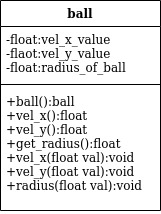
\includegraphics[scale=0.5]{ball.jpg}
    \caption{The ball class}
    \label{fig:ball class diagram }
\end{figure}
This class represents the moving ball used to destroy the bricks
\subsubsection{Attributes}
All of the class attributes are private
	\begin{itemize}
		\item float:vel\_x\_value\\ Represents the x speed component.
		\item float:vel\_y\_value\\ Represents the y speed component.
		\item float:radius\_of\_ball\\ Represents the radius of the ball. 
	\end{itemize}
\subsubsection{Methods}
	\begin{itemize}
		\item ball():ball \\Constructor.
		\item vel\_x():float \\vel\_x\_value getter.
		\item vel\_y():float\\vel\_y\_value getter.
		\item get\_radius():float\\ radius\_of\_ball getter.
		\item vel\_x(float val):void \\ vel\_x\_value setter.
		\item vel\_y(float val):void \\vel\_y\_value setter.
		\item radius(float val):void \\ radius\_of\_ball setter.
	\end{itemize}

\subsection{Bar}
\begin{figure}[h!]
    \centering
    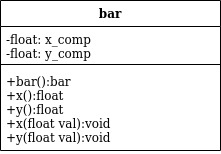
\includegraphics[scale=0.5]{bar.jpg}
    \caption{The bar class}
    \label{fig:bar class diagram }
\end{figure}
This class represents the moving bar controlled by the player
\subsubsection{Attributes}
All of the class attributes are private
	\begin{itemize}
		\item float: x\_comp\\Horizontal component of the distance between the bar center and the extremities.
		\item float: y\_comp\\Vertical component of the distance between the bar center and the extremities.
	\end{itemize}
\subsubsection{Methods}
	\begin{itemize}
		\item bar():bar\\Constructor.
		\item x():float\\x\_comp getter.
		\item y():float\\y\_comp getter.
		\item x(float val):void\\x\_comp setter.
		\item y(float val):void\\y\_comp setter.
	\end{itemize}
\newpage
\subsection{Game$\_$field}
\begin{figure}[h!]
    \centering
    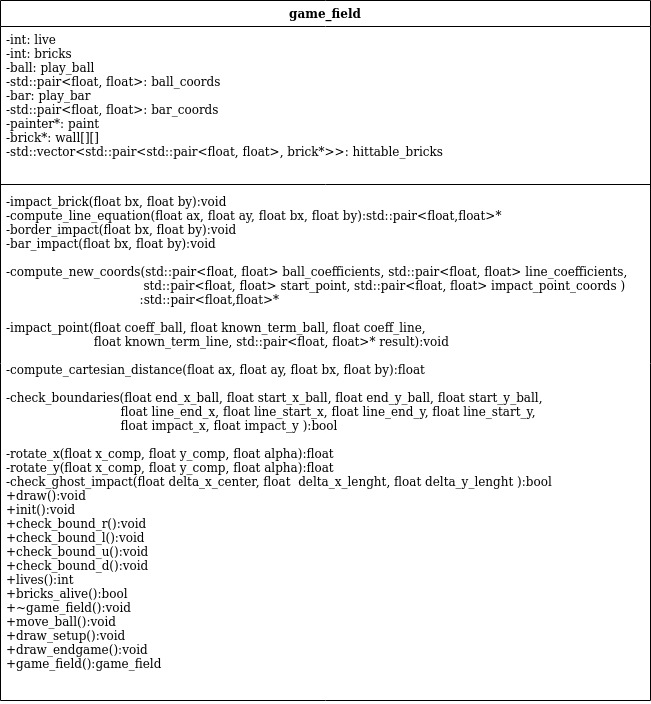
\includegraphics[angle=90, scale=0.5]{game_field.jpg}
    \caption{The game\_field class}
    \label{fig:painter game_field diagram }
\end{figure}
This class contains all the game object and the rules for their updates and interaction
\subsubsection{Attributes}
All of the class attributes are private
	\begin{itemize}
		\item int: live \\Represents the lives the player currently has.
		\item int: bricks \\Number of bricks still alive.
		\item ball: play\_ball \\Ball class instance.
		\item std::pair$<$float, float$>$: ball\_coords\\Coordinates of the ball.
		\item bar: play\_bar\\Bar class instance.
		\item std::pair$<$float, float$>$: bar\_coords\\coordinates of the center of the bar.
		\item painter*: paint \\ Pointer to a painter class instance, grants the possibility to represent data via the view.
		\item brick*: wall[ ][ ] \\Bidimensional matrix of references to the bricks on the playfield.
		\item std::vector$<$std::pair$<$std::pair$<$float, float$>$, brick*$>$$>$: hittable\_bricks \\ A vector of pairs whose first element are the indexes of the brick in the wall matrix and the second element is a pointer to said brick. This structure is used to represent the bricks that can be reached by the ball.
	\end{itemize}

\subsubsection{Methods}
	\paragraph{Private methods}
	\begin{itemize}
	\item impact\_brick(float bx, float by):void\\ This function is called to check wether the ball will hit any brick with its next movement. If it is so, ball coordinates and speed components will be updated accordingly, the brick will be hit and, if destroyed, the data structures will be updated accordingly.
	\item compute\_line\_equation(float ax, float ay, float bx, float by):std::pair$<$float,float$>$*\\Given two points this method will compute the coefficient and the known term of the line defined by those two points. Note that if the line is parallel to the y axis, the result returned will be (0,0). This doesn't lead to errors since, as the system has been built, the only time that a line of equation y=0 can be addressed is treated separetly in the method move\_ball(). .
	\item border\_impact(float bx, float by):void \\This method checks if, with the next movement, the ball will impact the sides or the ceiling of the playflield. If it is so, ball coordinates and speed component are updated accordingly.
	\item bar\_impact(float bx, float by):void \\This method checks if, with the next movement, the ball will impact with the bar. If it is so, the ball coordinates and speed components are updated accordingly.
	\item compute\_new\_coords(std::pair$<$float, float$>$ ball\_coefficients, std::pair$<$float, float$>$ line\_coefficients, std::pair$<$float, float$>$ start\_point, std::pair$<$float, float$>$ impact\_point\_coords )std::pair$<$float,float$>$*\\Given the line along which the ball moves, the line upon which the bar resides, the ball start point and the computed impact point this method computes the new coordinates of the ball.
	\item impact\_point(float coeff\_ball, float known\_term\_ball, float coeff\_line, float known\_term\_line, std::pair$<$float, float$>$* result):void \\Given the bar line and the ball line this method computes the impact point between the two lines.
	\item compute\_cartesian\_distance(float ax, float ay, float bx, float by):float\\This method computes the cartesian distance betweeen two points.
	\item check\_boundaries(float end\_x\_ball, float start\_x\_ball, float end\_y\_ball, float start\_y\_ball, float line\_end\_x, float line\_start\_x, float line\_end\_y, float line\_start\_y, float impact\_x, float impact\_y ):bool \\ Given the points defining 2 segments, the lines to which they lay on and the impact point between the two lines this method computes wether the impact point is within the boundaries of the segments. 
	\item rotate\_x(float x\_comp, float y\_comp, float alpha):float \\This method executes a rotation of alpha degrees on the x coordinates.
	\item rotate\_y(float x\_comp, float y\_comp, float alpha):float\\This method executes a rotation of alpha degrees on the y coordinates.
	\item check\_ghost\_impact(float delta\_x\_center, float  delta\_x\_lenght, float delta\_y\_lenght ):bool \\This method checks wether the bar will skip over the ball with its next movement. If it is so the method returns true.
	\end{itemize}

	\paragraph{Public methods}
	\begin{itemize}
		\item draw():void \\This method is called by ofApp during the game phase in order to print the state of the playfield. 
		\item init():void \\Initializes the class. Its main use is for it to be overloaded in future class extensions, since the initialization of this class is done in the constructor method.
		\item check\_bound\_r():void\\Checks if it is possible to move the bar right, also checking for ghost impacts. If the action is possible the data is updated accordingly.
		\item check\_bound\_l():void\\Checks if it is possible to move the bar left, also checking for ghost impacts. If the action is possible the data is updated accordingly.
		\item check\_bound\_u():void\\Checks if it is possible to rotate the bar counter-clockwise, also checking for ghost impacts. If the action is possible the data is updated accordingly.
		\item check\_bound\_d():void\\Checks if it is possible to rotate the bar clockwise, also checking for ghost impacts. If the action is possible the data is updated accordingly.
		\item lives():int\\Returns the number of lives left.
		\item bricks\_alive():bool\\Returns true if there is at least one brick left.
		\item ~game\_field():void\\Deallocates painter instance and cleans the pointers.
		\item move\_ball():void\\Moves the ball, checking for for all the different kinds of impacts and for life loss. Data is updated according to the results obtained.
		\item draw\_setup():void\\Calls the painter methods relative to the visual representation of the setup phase.
		\item draw\_endgame():void\\Calls the painter methods relative to the visual representation of the endgame phase.
		\item game\_field():game\_field\\Class constructor and initializer. The bricks are generated randomly everytime.
	\end{itemize}
\newpage
\section{Application workflow}
The application is controlled by the loop provided by OF thus entering setup() when the application starts; then the methods update and draw will alternate for the duration of the application execution time. When is time to terminate the applicationo the method ofBaseApp::exit() will be called.\\
In order to understand the algorithms there are two things worth noting:
\begin{itemize}
	\item The area on which the game elements sre positioned will be treated as a cartesian plain, with the origin at the bottom left corner, x coorddinates grow when moving to the right and y coordinates grow while moving upwards. The dimension of the field is hardcoded as 20 by 30.
	\item most of the times std::pair$<$float, float$>$ is used to represent points coordinates. The first element is the x coordinate and the second one is the y coordinate. 
\end{itemize} 
In this section will discuss the information flow and the apllication mechanisms in each of the three phases
\subsection{Setup phase}
As mentioned in the introduction, this is the state in whih the application starts. During this phase the player has the possibility to regulate the Kinect's angle by using the up and down arow keys. When one of these
two keys is pressed the method ofApp::keyPressed(int key) is called and, if the new angle is lesser than 30 and greater then -30 the cnages sre applied to the kinect.
The conditions on the angle are there in order to protect the kinect's motor from breaking while tryinng to reach unreachable positions.\\
Until the right arrow key is pressed the update() method simply refreshes the camera feed and prints the depth view on the screen, while the painter class is asked (via the playfield pointer) to print on the screen the instruction for the user, as well as an overlay over the kinect depth view to indentify visually the areas of interaction.\\
When the user presses the right arrow key the variable setup\_\_var is set to false, thus prompting the switch from the setup phase to the game phase.
\newpage
\subsection{Game phase}
The game phase constitues the most important and temporally long phase.\\
The first thing done is a check over the number of bricks left and of live left: if either of those is 0 the endgame variable is set to true and the control cycle will not be performed.\\
While in the game phase the controller alternates between updating the bar data unsing the kinect depth feed and prompting the updates on the ball position (and subsequent changes to the data) to the element pointed at by the playfield element.\\
Using the binary variable update\_cycle, the ofApp::update() method alternates between the two aformentioned activities
\subsubsection{update$\_$cycle==false}
When in this case the ofApp::update() method prompts the game\_field instance to move the ball by calling the method game\_field::move\_ball().\\
\paragraph{Hit bricks}
The first thing done during the execution of this method is to compute the new coordinates by adding to the current coordinates, contained in ball\_coords, by adding to the x coordinate the x component of the speed of the ball and by adding to the y coordinate the y componentof the speed of the ball.\\
If y component of the start point or of the end point are above the lower limit of the lowest row of bricks then it is possible that the ball will hit a brick on its trajectory, thus the method game\_field::brick\_impact is called, passing as parameters the coordinates of the ball after the movement.\\
The hittable\_bricks vector is then scanned, searching for impact points that are actually on the bricks, in the right direction and close enough to the ball to be reached. Of all the possible points the closest one is considered to be the right one.\\
If any impact is found the brick gets hit and the ball updates its speed components: if the brick was hit on the side then the x component is inverted, if instead the brick is hit onn the high or the low side the y component is inverted; while the ball position is updatedd according to the impact point.\\
\paragraph{Brick destruction}
If a brick gets destroyed its is\_alive attribute is set to false, then all the surrounding bricks in the wall matrix are evaluated: if a brick is adjacent, alive andd not hittable it is set as hittable and added to the hittable\_bricks vector.
Then the destroyed brick is erased from the hittable\_bricks vector.
\paragraph{Bar collision}
If no brick gets hit the coordinates of the ball won't change, thus a check on the ball\_coords is perfomed by game\_field::move\_ball. 
If the coordinates have changed the method returns, otherwise it calls the method bar\_impact, passing the ball coordinates after the movement as argouments. This method checks 
wether the ball will collide with the bar. This is done by computing the impact point of the two lines defined by the bar itself and by the ball speed.
If the computed impact point is invalid the method will return, otherwise a change of coordinates is done by performing a rotation, in order to find a x' axis parallel to the bar line.\\
The ball position are rotated accordingly, then the rotated y velocity is inverted and the counter rotation is performed, thus finding the new speed components.\\
The new ball coordinates are then computed by finding the intersection point between the ball speed line and the line paralle to the bar line and whose distance from the bar line is equal to the bar radius.\\
If one of the new speed components ends up being 0 it is incremented to a value slighly higher thn 0, in order to avoid getting the ball stuck on a trajectory.
\paragraph{Border collision}
If no bar hit is detected(once again by checking wether the ball has updated its coordinates), the border\_impact method is called, once again passing the computed new coorddinates as argouments.\\
The collisions with the border are checked analizing the argouments: if the x ccoordinate is $<$0 there is an impact on the left, if it is $>$20 there is an impact on the right and if the y component is $>$30 ther's an impact on the roof. \\
If a collision is detected the ball coordinates are updated accordingly and the speed gets modified (an impact no the left or the right prompts a x component inversion, while an impact on the roof promts a y component inversion).
\paragraph{Life lost}
If, again, the coordinates of the ball haven't changed a check is performed on the y component of the new coordinates: if it is lesser than 0 a life is lost and the speed and coordinates of the ball are reset. Otherwise the ball coordinates simply get updated and the method returns.    
\subsubsection{update$\_$cycle==true} 
In this situation the ofApp::update method will set the update\_cycle variable back to false and will then proceed to elaborate the Kinect feed
\paragraph{Centroid computation}
The algorithm will sample some points from the depth field and discard the ones that are not inside the desired range (from 1 meter to 1 meter and 15 centimeters). The coordinates of the undiscarded points are then averaged, thus obtaining the coordinates of the centroid of the cluster composed by valid points.\\
\paragraph{Command recognition}
The coordinates of the centroid are then compared to che coordinates of the center of the area seen by the kinect, plus or minus a treshold in order to grant a dead zone, both vertically and horizonatlly.
A high centroid will make the bar rotate counter-clockwise, a low one will make it rotate clockwise, a centroid on the left will make the bar move to the right and a centroid to the right will make the bar move to the left.
This is so since the Kinect depth feed is not specular, thus the lfet-right axis had to be inverted.\\
During the updates both the checks on the boundaries and the modifications to the bar attributes are performed
\paragraph{Ghost impact check}
In order to avoid the bar skipping over the ball and thus missing to register an impact a check is performed by rotating the coordinates to find the x' and x'' axis parallel to the bar before and after the rototrslation and analyzing the rotated coordinates of the ball before and after the rotostraslation.\\
If the ball is recognised to have skipped through the bar the rototraslation isn't allowed.
\subsubsection{Visual representation}
At each ofApp:draw execution the game\_field prompts the painter to uppdate the visual reepresentation, passing information about the bricks(whose colors change according to their lifepoints left), ball position, bar position and attributes and lives left.\\
The painter also draws the boundaries of the field and information about the meaning of the different brick colors.
\newpage
\subsection{Endgame phase}
In this phase the player has to choose wether to play again or to exit the application. This is done by using the arrow keys: up means the player wants to play again, down means the player wants to exit the game.
\subsubsection{New round}
When the up key is pressed both the variables chose and play\_again are set to true; thus ofApp::update will reset all the variables, delete the current game\_field instance and create a new one and the phase will go back to setup.
\subsubsection{Exit application}
When the down key is pressedd the fariable chose will be set to true, while the variable play\_again will be set to false; thus ofApp::update will delete the current playfield, close the Kinect feedd and exit the application.
\subsubsection{Video representation}
Painter will display a different message according to wether the player has won or has lost the game; it will also display the instructions on how to play again or exit the game  
\newpage
\section{User manual}
\subsection{Setup}
In order for the application to work OF is needed, as well as the OpenKinect libraries. The RADME file contains the links to their webpage, but a quick search on internet should get you there as well.\\
Once you have downloaded the repository from git, you need to move the application folder in the apps directory in the openframeworks folder, open the makefile and follow the instructions.\\
Open then the directory containing the makefile in a terminal and type "sudo make" to compile the release version. The sudo command is needed, otherwise it won't be possible to create the needed folders.\\
Once you have compiled the code, type "make RunRelease" to start the application (note that the command is case sensitive).
\subsection{Playing the game}
The Kinecct will be set to only consider objects between 1 meter and 1 meter and 15 centimeters of distance from the device, so during the setup take into consideration the distance at which the kinect stops seeing your hands.\\
Given how the code works you can use anything that can be picked up by the Kinect sensor to play.

\newpage
\section{Final remarks}
\subsection{References}
\begin{itemize}
	\item APSC slides and material for the academic year 2019-2020
	\item "A tour of C++", by Bjarne Stroustrup
	\item Openframeworks documentation and community support
	\item OFbook
	\item cppreference.com
	\item cplusplus.com
	\item OpenKinect documentation
\end{itemize}

\end{document}